%%%%%%%%%%%%%%%%%%%%%%%%%%%%%%%%%%%%%%%%%%%%%%%%%%%%%%%%%%%%%%%%%%%%%%%%%%%%%%%%%
%																				%
% ELEN4006 Project.tex														%
%																				%
%                       Ntsako Manyike (18 May 2011)							%
%																				%
%           Measurements Project								%
%                                                                               %
% Note: Minor modifications were made to the original paper                     %
%       by KJ Nixon 2005/10/12 (with permission from the original author        %
%																				%
%%%%%%%%%%%%%%%%%%%%%%%%%%%%%%%%%%%%%%%%%%%%%%%%%%%%%%%%%%%%%%%%%%%%%%%%%%%%%%%%%

\documentclass[10pt,twocolumn]{witseiepaper}

%
% All KJN's macros and goodies (some shameless borrowing from SPL)
\usepackage{KJN}
\usepackage{rotating}

%
% PDF Info
%
\ifpdf
\pdfinfo{
/Title (MEASUREMENTS PROJECT)
/Author (Ntsako Kennedy Manyike)
/CreationDate (D:201105180245)
/ModDate (D:201106040800)
/Subject (Final Report)
/Keywords ()
}
\fi

%%%%%%%%%%%%%%%%%%%%%%%%%%%%%%%%%%%%%%%%%%%%%%%%%%%%%%%%%%%%%%%%%%%%%%%%%%%%%%%
\begin{document}


\title{MEASUREMENTS PROJECT}

\author{Ntsako Manyike}

\thanks{School of Electrical \& Information Engineering, University of the
Witwatersrand, Private Bag 3, 2050, Johannesburg, South Africa}



%%%%%%%%%%%%%%%%%%%%%%%%%%%%%%%%%%%%%%%%%%%%%%%%%%%%%%%%%%%%%%%%%%%%%%%%%%%%%%%
%
\abstract{The design and construction of an electric microscope stage, powered
by an X-Y linear synchronous motor (LSM) is presented.  The system is to be
used to automate specimen photomicrography to effect rapid diagnoses of
illnesses.  The development of both motorised stage and its drive system is
discussed.  The drive system was tested using sinusoidal and pulse width
modulation (PWM) power signals. Tests showed that the combination of
wire-wound armature and PWM power signals provided the best performance.
However, slow, smooth motion could not be achieved, especially without
suitable closed-loop feedback.  It was concluded that the X-Y LSM layout used
was not ideal and a more suitable layout is presented which aims to improve
performance by using four independent linear synchronous motors.}

\keywords{Automated stage, LSM, microscope, X-Y linear motor}


\maketitle
\thispagestyle{empty}\pagestyle{empty}


%%%%%%%%%%%%%%%%%%%%%%%%%%%%%%%%%%%%%%%%%%%%%%%%%%%%%%%%%%%%%%%%%%%%%%%%%%%%%%%
%
\section{INTRODUCTION}

The diagnosis of many diseases, including Tuberculosis (TB) and Malaria,
requires the analysis of many sections of a specimen.  This system is not
perfect as irregularities in the specimen may congregate resulting in an
incorrect diagnosis.  For an accurate diagnosis, more sections of a specimen
need to be analysed.  Image recognition software exists to analyse digitised
images for patterns, which may represent contaminations.  A means of quickly
capturing images of a specimen for this computation to be performed is not as
common.  

To eliminate this bottleneck, an automated stage was developed.  Its
construction was based on the Olympus BX50 \cite{Olympus} and its automation
was provided by an X-Y LSM.  The BX50 is fitted with a manual stage and is
designed to host a light-weight, compact stage.

The capture rates of existing digital devices influenced the speeds at which
the stage moved.  Image recognition software requires computer resources, but
it was assumed that these facilities may not be available at the microscope
station.  Therefore the system was to be designed as a standalone system, with
optional computer control via an appropriate interface.

Success was based primarily on the achievement of smooth, speed-optimised X-Y
linear motion allowing clear images of the specimen to be captured.
Thereafter, a standalone, light-weight, compact and efficient design provided
measures of success.  The designed motorised stage and its drive system are
presented.  The performance is discussed and an alternative solution
presented.
%%%%%%%%%%%%%%%%%%%%%%%%%%%%%%%%%%%%%%%%%%%%%%%%%%%%%%%%%%%%%%%%%%%%%%%%%%%%%%%%
\section{BACKGROUND}

\subsection{Disease diagnosis}

The diagnosis of Tuberculosis and Malaria involves the examination of sputum
and blood samples respectively \cite{phppo,biotec,STimes}.  These examinations
also reveal the contagious quality of infections such as TB.  Therefore,
faster diagnosis results in better containment of the disease and allows the
patient to be treated before their condition worsens.  This is of particular
importance when one considers the consequences associated with a delayed
diagnosis of an AIDS patient.  AIDS disables the immune system.  A patient
dies from a secondary infection such as Malaria or TB.  The scale of the
problem is of significance.  Tuberculosis has been listed as a global problem
by the World Health Organisation \cite{biotec}.  The National University
of Singapore has used image recognition software to analyse digitised
microscope images to diagnose Malaria with greater speed than
before \cite{STimes}.  Besides providing a faster means of performing
diagnoses, the project provides less qualified medical technicians with a
means to perform the diagnoses.

%%%%%%%%%%%%%%%%%%%%%%%%%%%%%%%%%%%%%%%%%%%%%%%%%%%%%%%%%%%%%%%%%%%%%%%%%%%%%%%
\subsection{Microscope stages}

A microscope stage is required to move along all three axes.  The vertical
motion of the stage provides a focusing mechanism and is usually performed by
moving the stage mounting system vertically.  The specimen is then moved in
the X-Y plane, about the optical centre of the microscope stage, exposing any
point of the specimen to the viewer.  On the Olympus BX50, this motion is
provided by two concentric rotary dials.

\subsubsection*{Existing automated microscope stages:}

The automation of microscope stages has been performed by various companies.
Geared rotary stepper motors and piezo electric linear motors have been used
to provide this linear X-Y motion.  Each is suited to a particular
application.

The rotary stepper motor solution is the most common solution.  They provide
micrometer resolution with a relatively compact design and easy control and
drive system.  Olympus \cite{Olympus}, Prior Scientific \cite{Prior} and Applied
Scientific Instrumentation \cite{Ms4} have stages on the market that make use
of this technology, for standard microscope applications.

For nanotechnology, the piezo linear motors produced by PI \cite{PI} are
incorporated into an automated stage.  The application of a voltage to the
piezo-electric crystals causes them to bump the stage along with a resolution
of 50 pm and a range of 1 mm.  This low range allows for capacitive sensors to
provide accurate positional feedback.

Additional options and features offered by these manufacturers include
joystick control and RS-232 control.  The simplest of systems, suited to the
Olympus BX50, range between R40 000 and R50 000 from a local
supplier \cite{Elmulab} or from between R16 000 and \mbox{R35 000} excluding
shipping charges from Prior Scientific, UK \cite{Prior}. 

%%%%%%%%%%%%%%%%%%%%%%%%%%%%%%%%%%%%%%%%%%%%%%%%%%%%%%%%%%%%%%%%%%%%%%%%%%%%%%%
\subsection{Digital camera systems}

The Olympus BX-50 has adopted standard photomicrography camera lenses, namely
C- and CS-mounted lenses \cite{Olympus}.  The capture rate of available
digital capture devices range between 1/60 fps, from still cameras, to 30 fps,
from video cameras using the National Television Standards Committee (NTSC)
system \cite{Olympus}.

%%%%%%%%%%%%%%%%%%%%%%%%%%%%%%%%%%%%%%%%%%%%%%%%%%%%%%%%%%%%%%%%%%%%%%%%%%%%%%%
\subsection{Linear synchronous motors}

LSM's have come into favour because of \cite{Halbach-1,XY-Thrust}:
\begin{enumerate}
	\item Their accurate positioning capabilities via DC excitation.
	\item The lower cost and weight of permanent magnet (PM) movers which do not require power supplies
	\item The high thrusts, speeds and efficiencies they can provide.
	\item The absence of a transmission which eliminates gearing losses, and increases reliability and dynamic performance.
\end{enumerate}

%%%%%%%%%%%%%%%%%%%%%%%%%%%%%%%%%%%%%%%%%%%%%%%%%%%%%%%%%%%%%%%%%%%%%%%%%%%%%%%
\section{SYSTEM DESIGN}

\begin{figure}[ht]
	\centering
		
\includegraphics[width=0.45\textwidth]{../../Drawings/Flow-Diagram.pdf}
	\caption{System Overview}
	\label{fig:Sys}
\end{figure}
\figref{fig:Sys} depicts the three sections of the designed system.

\subsection{dsPIC30F6014 microcontroller unit}
The dsPIC30F6014 MCU \cite{Microchip} was used to control the motor.  In the
case of sinusoidal power signals, it presented digital signals to two
digital-to-analog converters (DAC).  For the application of PWM power signals,
six output-compare channels were used.
 
\subsection{Drive system electronics}

\subsubsection*{Sinusoidal Power Signals:}
Two 12-bit DAC's produced the A and C phases for both directions.  A sequence
of inverting summing amplifiers generated the third phase from the redundancy
in three-phase systems, and provided bipolar operation.  Six Class-AB power
amplifiers provided the current necessary to drive the X-Y LSM.

\subsubsection*{PWM Power Signals:}
A six channel class-D amplifier provided the current necessary to drive the
X-Y LSM through a filter bank. The filter bank was developed to compensate for
the armature's low filtering ability.

\subsection{X- and Y- direction windings}

The armature windings were based on two flat, stacked, orthogonal LSM's as
described by Davies \cite{Simon}, providing independent two-dimensional
movement.

%%%%%%%%%%%%%%%%%%%%%%%%%%%%%%%%%%%%%%%%%%%%%%%%%%%%%%%%%%%%%%%%%%%%%%%%%%%%%%%
\section{STAGE DESIGN}

\begin{figure}[hb!]
	\centering
		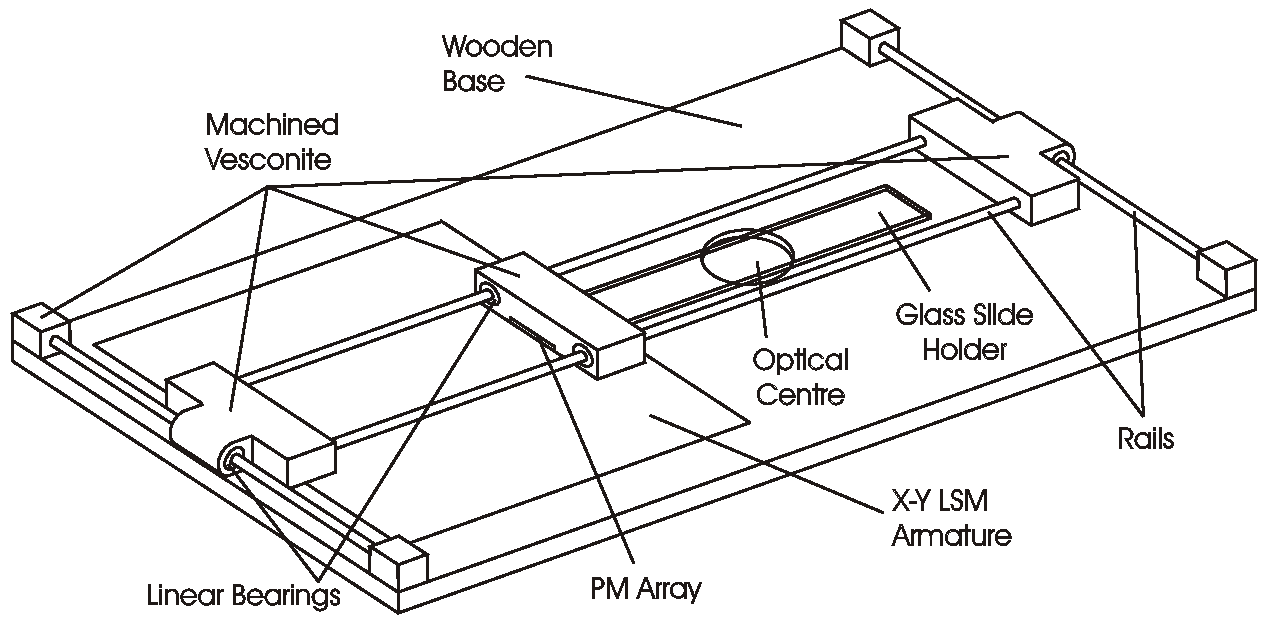
\includegraphics[width=0.50\textwidth]{../../Drawings/Stage-Final.pdf}
	\caption{Stage Design}
	\label{fig:Stage}
\end{figure}
%Placed Here so as to appear correctly
\begin{table*}[ht!]
	\centering
	\caption{Armature Advantages and Disadvantages}
		\begin{tabular}{lll}
			\hline
													&	{\msbf Advantages} 						& {\msbf Disadvantages}\\
			\hline
			{\msbf PCB}					& 1) The thin armature reduced leakage  			& 1) 24 series-turns/phase; costly to increase\\
													& flux and eliminated LSM vertical separation.& 2) High Cost (R3 000)\\
													& 2) The pole-pitch was exactly matched.\\													
			\hline
			{\msbf Wire-Wound}	& 1) Low Cost (R200)										& 1) Thicker armature increased leakage\\ 
													& 2) 180 series-turns/phase			& flux and imposed vertical LSM separation.\\
													& 3) Well matched pole-pitch  	& 2) Timely construction procedure.\\						\hline
		\end{tabular}
	\label{tab:Armatures}
\end{table*}
The stage in \figref{fig:Stage} was constructed from a machined wooden base.
This material provided the lowest cost and weight when compared to metallic or
plastic materials.  It hosted the sunken armature which was offset from the
optical centre of the stage.  It was offset to allow the light to pass through
the stage unobstructed, and sunken to allow the railing system to be fitted as
low as possible.  This provided the closest possible suspension of the PM
array, increasing flux linkage.  Excessive height also reduces the
microscope's focusing range.  The railing system consisted of 5 mm diameter
silver steel rails on which IKO LBE5 linear bearings were run.  The bearings
were encased in machined Vesconite, which also served to hold the rails in
place, aligned to within 0.01 mm at the ends.  A 3 mm thick piece of glass was
fitted into the bottom of the central mover, providing a surface on which the
specimen could be placed.  The cursor PM array was fitted onto the glass,
directly below the central mover.  This prevented the vertical forces on the
PM from generating torques on the central mover's linear bearings, allowing
them to move smoothly. 

\subsection{LSM design}

The layout specified by Davies \cite{Simon} was scaled for use in this
application.  The LSM's orthogonal placement provided independent motion along
two dimensions because of the associated orthogonal magnetic fields and
theoretical zero mutual inductance.  The disadvantage of this layout was that
the individual LSM's were at different depths from the cursor.  The result was
that, at the level of the PM array, the lower LSM produced a weaker magnetic
field than the upper LSM.

The armature was a slotless design.  Although the magnetic field was weaker in
this design, the detent forces were eliminated \cite{Tubular,XY-Thrust}.
Detent forces are the periodic attractive forces between the PM's and the
metallic slots between the windings.  In order to achieve smooth motion, these
forces must be eliminated.  

The LSM was a single sided design, employed to minimise the height of the
system.  The disadvantage of this design was that less flux was
generated \cite{Linsync}.  A back iron was also neglected because of the
associated weight which could not be accommodated by the stage support.  This
reduced flux linkage.

The topology employed consisted of an active armature and a passive PM
cursor \cite{Linsync}.  The advantage of this topology was that the cursor was
electrically isolated from the stage such that no electrical contacts were in
motion.  This increased durability.

To determine the pole-pitch, the speeds required must be considered.  From the
Olympus BX50's technical data, the observable fields-of-view range between
0.22 mm and 5.5 mm.  From this, and the rate of capture of the digital imaging
devices, the linear speeds at which this system can move are between 0.176
mm/s and 44 mm/s.  This includes a 20\% overlap which allows for accurate
digital knitting.

To achieve these low speeds, minimisation of both the pole-pitch and the input
frequencies is essential.  The relationship between these three variables is
given in \eqnref{eqn:Speed}.  The pole-pitch was limited by the dimensions of
available Nd-Fe-B PM's.  The smallest available PM's were \mbox{8.6 $\times$
8.6 mm $\times$ 3 mm}, polarised along their shortest dimension. To minimise
force-ripple, the ratio of the magnet-length to the machine pole-pitch is
0.8 \cite{Tubular}.  This ratio results in reduced harmonics in the DC magnetic
field and lower thrust, but is essential for smooth motion. Therefore, the
system pole-pitch was 10.75 mm and the excitation frequencies needed to be
between 0.008 Hz and 2 Hz.
\begin{equation}
	v = v_s = 2f\tau
	\label{eqn:Speed}
\end{equation}
where:

\begin{tabular}{lll}
& $v$      & = Linear Velocity (mm/s)\\
& $v_s$    & = Synchronous Linear Velocity (mm/s)\\
& $f$      & = Input Frequency (Hz)\\
& $\tau$   & = Pole Pitch (mm) \\
\end{tabular}

Two armatures were tested.  The first design made use of a PCB.  The second
was a wire-wound armature.  The advantages and disadvantages of both are
presented in \tabref{tab:Armatures} with a final specification given in
\tabref{tab:Specs}.  The two PM arrays shown in \figref{fig:PM} were also
tested.  They represent compromises between size and flux linkage.
%Placed Here so as to appear correctly
\begin{table}[hb!]
	\centering
	\caption{Motor Specifications}
		\begin{tabular}{lll}
			\hline
           	 & {\msbf Specification} 	& {\msbf Value (Units)}\\
      \hline
          1. & 3$\Phi$ Connection   & $\Delta$\\
          2. & Pole Pairs							 & 6$\times$6\\
          3. & Pole Pitch							 & 10.75$\times$10.75 (mm)\\
          4. & PCB Track Width				 & 0.695 (mm)\\
          5. & PCB Series-Turns/Phase  & 24$\times$24\\
          6. & Wire-Wound wire $\oslash$   & 0.35 (mm)\\
          7. & Wire-Wound 						 & 180$\times$180\\
             & Series-Turns/Phase\\
          8. & Max Current   					 & 1.5 (A)\\
      		9. & Nd-Fe-B PM Size				 & 8.6$\times$8.6$\times$3 (mm)\\
      \hline
		\end{tabular}
	\label{tab:Specs}
\end{table}
\begin{figure}[htb!]
	\centering
		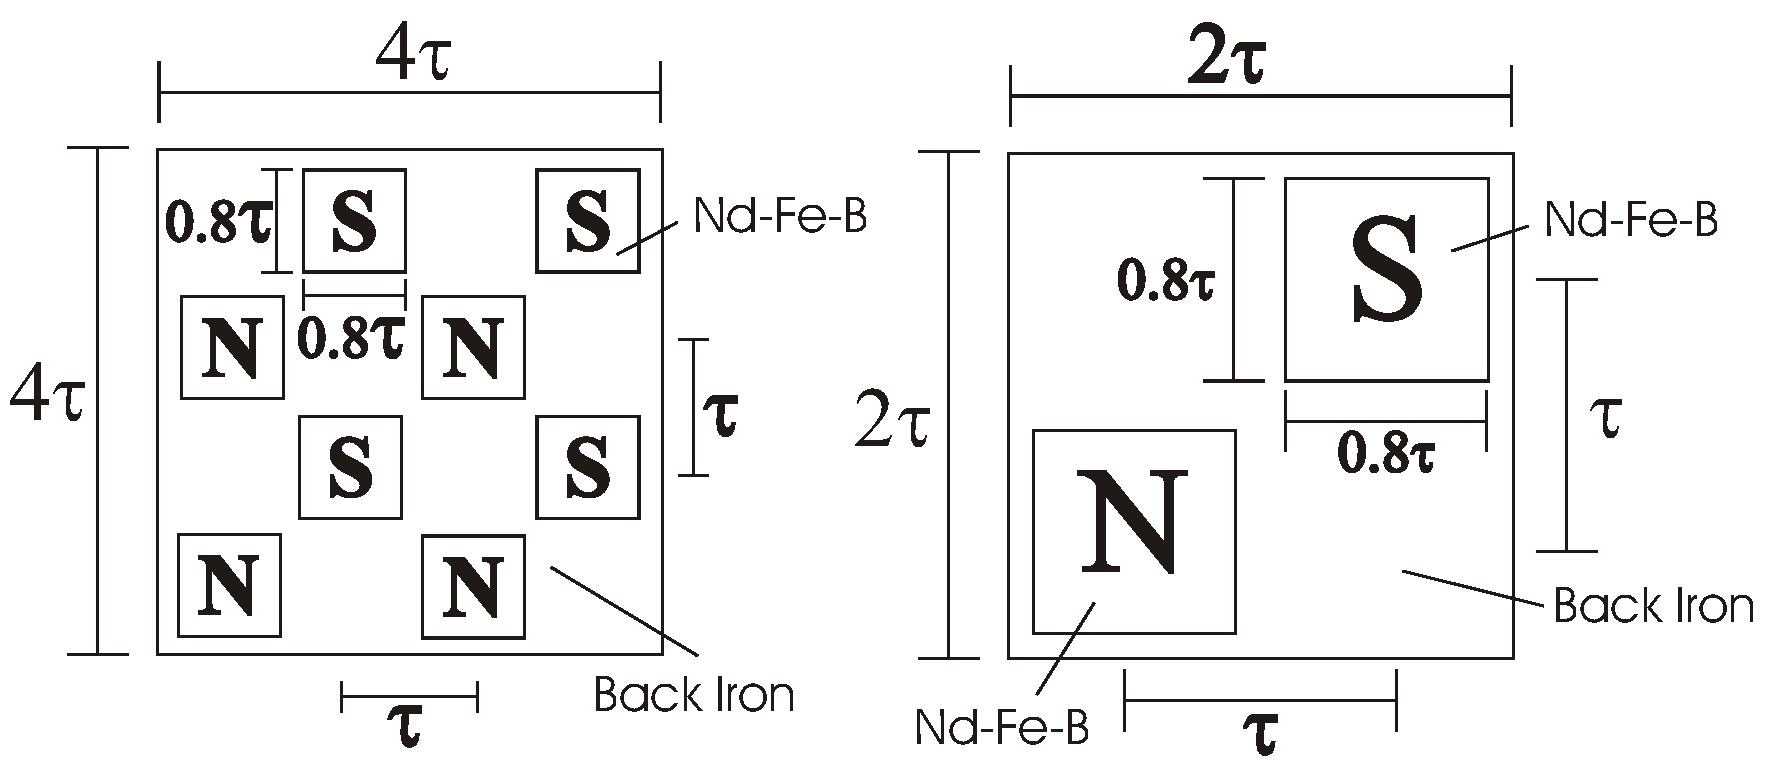
\includegraphics[width=0.48\textwidth]{../../Drawings/PM-Both.pdf}
	\caption{PM Array Configurations}
	\label{fig:PM}
\end{figure}
%%%%%%%%%%%%%%%%%%%%%%%%%%%%%%%%%%%%%%%%%%%%%%%%%%%%%%%%%%%%%%%%%%%%%%%%%%%%%%%
\section{DRIVER SYSTEM}
\subsection{dsPIC30F6014 microcontroller}
The dsPIC MCU was used to generate the six phase signals required to drive
both dimensions of the X-Y LSM.  The program strategy was designed according
to a layered system.  The signal generation formed the lowest level of the
structure and accepted two inputs, the X- and Y-direction frequencies, called
the frequency bus.  Subsequent layers existed separately from the generation
layer.  To control the LSM, a layer asserted a value onto the frequency bus.
This provided a means of stacking various layers such as a joystick or RS-232
controller layer.  

A 12-bit sampled sinusoid was stored in the program memory using the Page
Space Visibility functionality which allowed program memory to be accessed as
if it were data memory.  The generation layer accepted the two values on the
frequency bus and set up timers to interrupt accordingly.  On each timer
interrupt, the next value for each phase was read from the sinetable using
pointers.  For sinusoidal power signals, these values were written to the
12-bit dual DAC's using two 12-bit data buses and one 2-bit control bus.  For
the PWM power signals, these values represented the duty-cycles of the PWM
signals and were written into appropriate PWM registers.  The PWM signals ran
at a chopper frequency of 1.8 kHz.  This allowed for 12-bit resolution at the
available clock frequency.  Open-loop scalar control was implemented.  The
methodology of the MCU is illustrated in \figref{fig:Controller}.
\begin{figure}[hb]
	\centering
		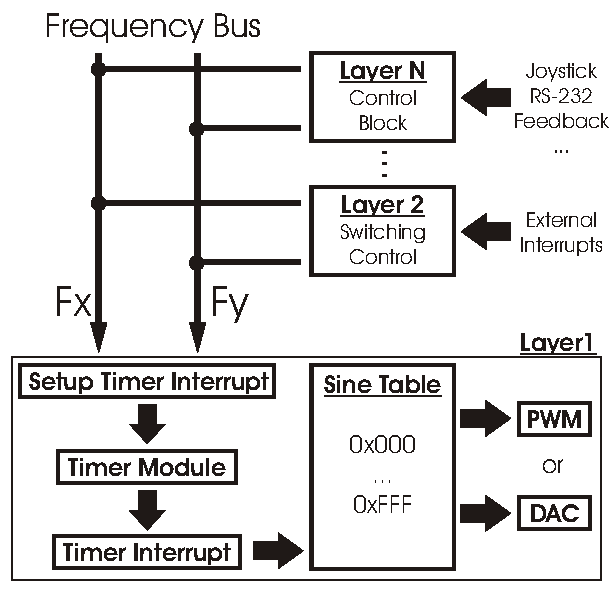
\includegraphics[width=0.45\textwidth]{../../Drawings/Controller.pdf}
	\caption{Controller Methodology}
	\label{fig:Controller}
\end{figure}
\subsection{Drive system electronics}

\subsubsection*{Sinusoidal power signals:}
The two 12-bit digital buses were connected to two Maxim MX7847BN DAC's.
Channel A of the two DAC's produced phases A and C for the X-direction whilst
Channel B produced the same for the Y-Direction.  Bipolar operation was
achieved using inverting, summing, operational amplifier configurations
according to the application notes.  For each direction, phases A and C were
summed in an inverting configuration to produce phase B according to
\eqnref{eqn:3Phase}.  Tuning potentiometers were set to within 0.2\% fullscale
(FS) to achieve phase and amplitude symmetry.  The six phase signals formed
inputs to the six current gain amplifiers.  These were class-AB power
amplifier configurations using TIP122 and TIP125 complimentary darlington
transistor pairs.  They could be driven directly from the TL074 op-amps
because of their high current gain ($H_{fe-min}=1000$).  This eliminated
excessive external circuitry.  A TL074 op-amp was used to ensure accurate
amplification by placing the class-AB amplifier in the feedback loop of the
op-amp, with a buffered input to the op-amp.  The six outputs were connected
directly to the X-Y LSM windings.  \begin{eqnarray}
	i_A+i_B+i_C = 0\nonumber\\
	i_B = -i_A-i_C\label{eqn:3Phase}
\end{eqnarray}
\subsubsection*{PWM power signals:}
The six TTL logic level PWM signals formed inputs into a six channel class-D
amplifier.  This consisted of a primary stage in which comparators, made from
TL074 op-amps, pushed the voltage signals to the rails.  Thereafter, the same
TIP122 and TIP125 complimentary darlington transistor pairs were used in an
H-bridge configuration to provide current amplification.

It is typically understood that the armature windings filter Voltage Source
Inverter PWM signals to produce smoothed current signals.  In reality, the
-3 dB frequency of the filter created by the armature windings is given by
$f=\frac{R}{2\pi L}$.  For the designed armatures, the resultant -3 dB
frequencies were 3.183 kHz and 17.683 kHz for the wire-wound and PCB armatures
respectively.  Therefore, the switching frequency permeated through the
armatures as current signals with no attenuation.  A six channel filter bank
was designed to compensate for this effect.  Each channel was a second order
RLC filter, as shown in \figref{fig:Filter}.  The resulting -3 dB frequency was
112 Hz.

\begin{figure}[hb]
	\centering
		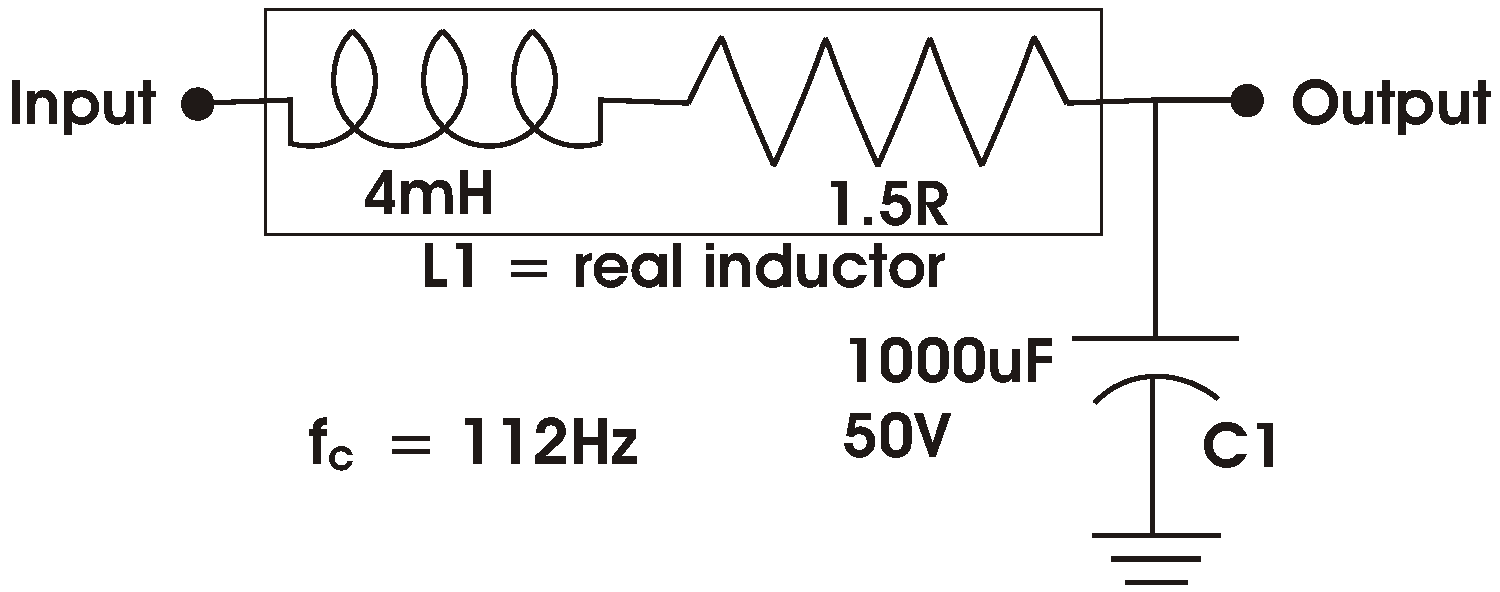
\includegraphics[width=0.45\textwidth]{../../Drawings/Filter.pdf}
	\caption{RLC Filter Circuit}
	\label{fig:Filter}
\end{figure}
%%%%%%%%%%%%%%%%%%%%%%%%%%%%%%%%%%%%%%%%%%%%%%%%%%%%%%%%%%%%%%%%%%%%%%%%%%%%%%%%%
\section{RESULTS}

Smooth motion was not achieved.  The contributing factors are considered below.

\subsection{Torsional effects}

Motion across the width of the stage was significantly more hap-hazard than
that of the movement along the stage's length.  The layout and placement of
the LSM resulted in the forces being applied at a distance from the linear
bearings.  The distance at which this force was applied was different for each
bearing, resulting in different torques on these bearings.  The resultant
torsional effect, when combined with frictional variations on each bearing,
would mis-align the bearings and cause them to cease.  The bearings were
released from this state once the cursor had slipped a pole and was pushed
backward for a short distance.  This effect was due to the offset positioning
of the LSM.  Not only was this a hindrance to smooth motion, but it was also
impractical in terms of it's spacial integration into a microscope system.

\subsection{Frictional effects at low speeds}

The linear bearings have extremely low frictional coefficients.  The static
coefficient is, as is typical, higher than the kinetic coefficient.  As the
magnetic wave built up behind the PM array, the force increased to overcome
the static friction.  When the force had become substantial enough to overcome
this friction, the cursor was thrust forward.  Because the frictional
coefficient had reduced, the resultant force increased in the direction of
movement.  The cursor moved suddenly, whilst the magnetic wave did not and
thus did not reinforce the original force that was applied to the cursor.
Therefore the cursor stopped and was once again affected by static friction.
The cycle began again, resulting in periodic motion.

\subsection{LSM construction}

The layout of the LSM contributed in many ways to the failure to achieve
smooth motion.  The wire-wound solution produced better results.

\subsubsection*{PCB armature:} 
The PCB design provided a solution whereby leakage flux was reduced, because
of the reduced air-gap associated with a thinner armature relative to the
pole-pitch.  The differing strengths of the X- and Y-direction windings at the
PM level were eliminated because of the alternate layering of X- and
Y-windings.  This design's major downfall was that, because of construction
costs and complexities, only 24 series-turns per phase could be accommodated
in the design.  In testing, the magnetic field produced could not overcome the
inertia of the railing system.

\subsubsection*{Wire-wound armature:}
The wire-wound armature produced a strong magnetic field and was able to
overcome the inertia of the railing system.  A 2.5 mm separation existed
between the X- and Y-direction windings because of its construction.  The
differing strengths of the magnetic fields were evident.  This design was able
to accommodate 180 series-turns per phase resulting in a 650\% increase in
efficiency over the PCB design.  The system still sourced 2 A from the power
supply making it inefficient.  The high currents however may be attributed to
the extra current needed to overcome the frictional and torsional effects.

\subsubsection*{Cursor design:}
The two-magnet design did not offer enough flux linkage to move the cursor
successfully.  The eight-magnet design worked, but with the obvious spacial
consequences.  Smooth motion may have been affected by the harmonics in the DC
magnetic field.

\subsection{Sinusoidal vs. PWM power signals}

The natural PWM power signals performed more effectively than the sinusoidal
power signals.

\subsubsection*{Sinusoidal power signals:}
These signals were highly susceptible to EMI and other sources of noise.  The
amplification of these signals was inefficient because of the linear
electronics involved.  The design was flawed by the inability to achieve phase
and amplitude symmetry.  The finite resolution of 0.2\% FS in the tuning
circuit resulted in an unbalanced three phase system.  When driving the X-Y
LSM with this imbalance, high-frequency noise was observed and is analogous to
two ocean waves crashing into one another.  

\subsubsection*{PWM power signals:}
The application of PWM power signals was efficient because the saturated
transistors present little resistance in the current path and hence dissipate
less energy, requiring smaller heatsinking components.  The electronic
circuitry was significantly less complex and less susceptible to high
frequency noise because of the digital nature of the signals.  The use of PWM
at the suitably high enough chopper frequency of 1.8 kHz provided a better
balanced sinusoidal system after the effective filtering of the filter bank.
The chopper frequency was attenuated by 54 dB, in the current waveform, by the
filter bank.

%%%%%%%%%%%%%%%%%%%%%%%%%%%%%%%%%%%%%%%%%%%%%%%%%%%%%%%%%%%%%%%%%%%%%%%%%%%%%%%%%
\section{DISCUSSION}

Smooth motion was not achieved since the layout of the X-Y LSM caused
torsional effects.  The low speeds required by the application caused
staggered motion due to the dynamics of the frictional forces in the system.
The efficiency was low due to the low 180 series-turns per phase resulting in
2 A being drawn from the power supply.   PWM power signals proved more
effective in maintaining phase and amplitude symmetry as opposed to sinusoidal
power signals.  However, this method required external filter banks ($f_c=112$
Hz to compensate for the ineffectual filtering ability of the armature.  The
stacked layout of the X-Y LSM prevented more series-turns from being built
into the system, whilst maintaining the low pole-pitch, because it separated
the lower windings from the PM array accordingly.  The wire-wound armature was
a better solution than the PCB design as it could accommodate more
series-turns per phase at a lower cost.  Therefore, in this layout, the
pole-pitch and ampere-turns necessary to provide smooth motion efficiently
could not be accommodated.
\begin{figure}[htb]
	\centering
		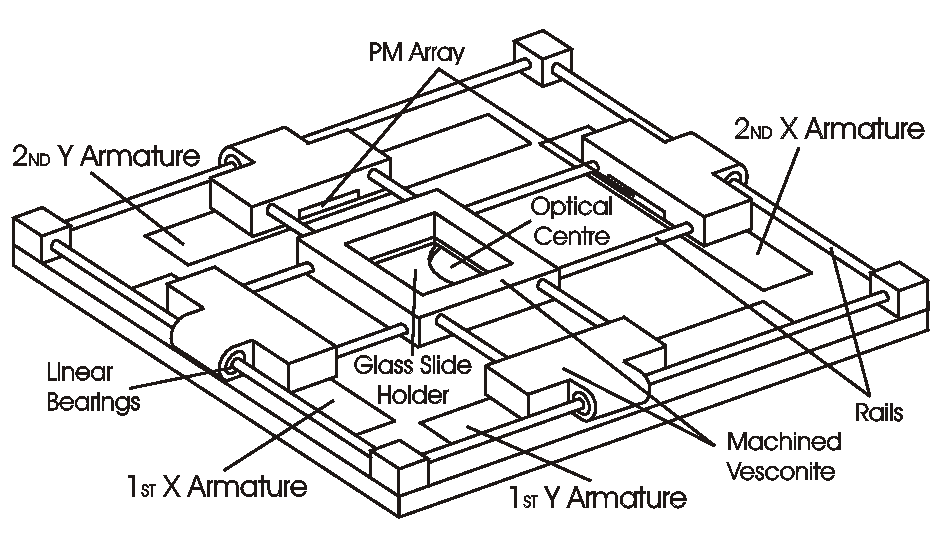
\includegraphics[width=0.48\textwidth]{../../Drawings/Future-Stage.pdf}
	\caption{Recommended Stage}
	\label{fig:Recommend}
\end{figure}
\vspace{-8mm} % SiS! KJN, but needed to make it look neat

An improved solution is depicted in \figref{fig:Recommend}, where four
individual LSM's are used, two for each dimension.  They are placed below
the linear bearings, under which the PM array is housed.  This prevents any
torsional effects from mis-aligning the bearings because adjacent LSM's are
excited from the same source.  Halbach arrays are recommended to increase flux
linkage with the armature, making large PM arrays unnecessary.  They will also
increase efficiency, accuracy and dynamic response resulting from their
sinusoidal magnetic field pattern \cite{Halbach-1,XY-Thrust}.  This new layout
also allows the stage to fit centrally about the optical centre, without an
offset motor.  The railing system is maintained as it helps improve efficiency
by reducing friction.  A suitable vector control strategy should be
implemented to achieve the desired smooth motion.  By separating the X- and
Y-direction windings, more ampere-turns can be accommodated by building in
further depth into each LSM.  This is done while maintaining the small
pole-pitch, if not reducing it simultaneously, depending on the availability
of Nd-Fe-B magnets.

%%%%%%%%%%%%%%%%%%%%%%%%%%%%%%%%%%%%%%%%%%%%%%%%%%%%%%%%%%%%%%%%%%%%%%%%%%%%%%%%%
\section{CONCLUSION}

Slow and smooth motion necessary for the automation of specimen
photomicrography could not be achieved due to torsional effects introduced
when only two X-Y linear synchronous motors were used to automate an electric
microscope stage. To resolve this problem, it is recommended that a layout
using four independent linear synchronous motors be implemented.


%%%%%%%%%%%%%%%%%%%%%%%%%%%%%%%%%%%%%%%%%%%%%%%%%%%%%%%%%%%%%%%%%%%%%%%%%%%%%%%%%
\section*{ACKNOWLEDGEMENT}

The author would like to thank Mr. H. Fellows, Mr. A. van Zyl and Mr. S.Q.
Davies from the School of Electrical and Information Engineering for their
guidance, and Mrs. E. Marais from the Wits Medical School for providing access
to the Olympus BX50.
%%%%%%%%%%%%%%%%%%%%%%%%%%%%%%%%%%%%%%%%%%%%%%%%%%%%%%%%%%%%%%%%%%%%%%%%%%%%%%%%%
%\nocite{*}

\bibliographystyle{witseie}
\bibliography{references}

%%%%%%%%%%%%%%%%%%%%%%%%%%%%%%%%%%%%%%%%%%%%%%%%%%%%%%%%%%%%%%%%%%%%%%%%%%%%%%%


%{\tiny \vfill \hfill \today \hspace{5mm} witseie-paper-2003.\TeX}

\end{document}

" vim: ts=4
" vim: tw=78
" vim: autoindent
" vim: shiftwidth=4

